\chapter{Análisis Vectorial}

Hasta ahora, probablemente poseen una familiaridad trabajando con coordenadas cartesianas en el espacio $\mathbb{R}^3$. Para definir un punto en este sistema, utilizamos las coordenadas $(x,y,z)$, que corresponden a la proyección del vector posición $\x$ sobre cada uno de los ejes cartesianos, rectas perpendiculares entre sí. Si mantenemos constante una de estas coordenadas, definimos un \emph{plano} perpendicular al eje que se ha mantenido constante. 

De esta forma, un punto $P$ con coordenadas $(a,b,c)$ corresponde también a la intersección de los planos $x=a$, $y=b$, $z=c$, perpendiculares a los ejes $x$, $y$ y $z$, respectivamente.

En este sistema, superficies más generales pueden describirse implícitamente mediante expresiones del tipo $F(x,y,z) = c$, donde $c$ es un valor constante. Por ejemplo, una esfera de radio $R$ puede ser descrita por la expresión $x^2+y^2+z^2 = R^2$. Distintos valores de $c$ permiten describir una \emph{familia} de superficies, con la misma naturaleza, pero diferentes posiciones.

Antes de entrar más de lleno en la discusión, recordemos e introduzcamos algunas definiciones.

\begin{defi} \marginnote{Delta de Kronecker}
    Se denomina \textbf{delta de Kronecker} al elemento $\delta_{ij}$, definido en un espacio vectorial de $n$ dimensiones como
    \begin{equation}
        \delta_{ij} = \begin{dcases}
            1, \qquad i = j \\
            0, \qquad i \neq j
        \end{dcases} \ .
    \end{equation} 

    Este elemento puede representarse de forma matricial como la matriz identidad del espacio de dimensión $n$.
\end{defi}

\newpage

\begin{defi} \marginnote{Base ortonormal}
    Sea un conjunto de vectores unitarios $\left\{ \hat{e}_i\right\}_{i=1}^n$ de un espacio $n$-dimensional. Diremos que este forma una \textbf{base ortonormal} si al realizar el producto escalar entre elementos del conjunto, se cumple la relación
    \begin{equation}
        \hat{e}_i\cdot \hat{e}_j = \delta_{ij} \ ,
    \end{equation}
    donde $\delta_{ij}$ es la delta de Kronecker.
\end{defi}

\begin{defi} \marginnote{Vector posición}
    Dado un sistema coordenado en un espacio de $n$ dimensiones, podemos definir el \textbf{vector posición} $\vec{x}$, que une el origen del sistema con punto con coordenadas $x_i$, con $i = 1, 2, \dots, n$ como
\begin{equation} \label{eq:vector-posicion}
    \vec{x} = x_1 \hat{e}_1 + x_2 \hat{e}_2 + \dots + x_n \hat{e}_n = \sum_{i=1}^n x_i \hat{e}_i \ ,
\end{equation}
donde las \textbf{componentes del vector} en la base $\{ \hat{e}_i\}_{i=1}^n$ pueden expresarse como
\begin{equation}
    x_i = \vec{x} \cdot \hat{e}_i \ .
\end{equation}
\end{defi}

Durante este capítulo, nos limitaremos a trabajar en tres dimensiones, pues son las necesarias para describir la gran mayoría de los fenómenos físicos que pueden interesarnos.

\section{Coordenadas curvilíneas ortogonales}


Supongamos que existen tres superficies descritas por las ecuaciones
\begin{equation}
    q_1(x,y,z) = c_1 \, , \quad q_2(x,y,z) = c_2 \, , \quad q_3(x,y,z) = c_3 \ ,
\end{equation}
que se intersectan en el punto $P=(a,b,c)$. Es decir, la única solución que satisface simultáneamente las ecuaciones anteriores es $(x,y,z) = (a,b,c)$.

Si las funciones $q_i$ son monovaluadas y con derivadas continuas, entonces estas serán invertibles, y podremos definir una correspondencia entre las coordenadas cartesianas $(a,b,c)$ y los valores $(c_1,c_2,c_3)$.

\begin{defi}
    Se denominan \textbf{superficies coordenadas} a las funciones de la forma
    \begin{equation}
        q_i(x,y,z) = c_i \ ,
    \end{equation}
    donde $i = 1, 2, 3$, cuya intersección define un \textbf{sistema de coordenadas curvilíneas} $(q_1, q_2, q_3)$.
    
    % un punto $P$, con \textbf{coordenadas curvilíneas} $(q_1, q_2, q_3)$.

    Si la intersección es en ángulo recto \emph{para todos los puntos}, se dice que el sistema es \textbf{ortogonal}.
\end{defi}

De esta forma, dado un punto $P$ con coordenadas cartesianas $(a,b,c)$, y con coordenadas curvilíneas $(c_1, c_2, c_3)$, podemos establecer la relación 
\begin{equation}
    x(c_1, c_2, c_3) = a \, , \quad y(c_1, c_2, c_3) = b \, , \quad z(c_1, c_2, c_3) = c \ ,
\end{equation} 
y el vector posición $\x(x,y,z) = x \hat{\imath} + y \hat{\jmath} + z \hat{k}$ podrá expresarse como 
\begin{equation*}
    \x(q_1, q_2, q_3) = x(q_1, q_2, q_3) \hat{\imath} + y(q_1, q_2, q_3) \hat{\jmath} + z(q_1, q_2, q_3) \hat{k} \ .
\end{equation*}

¿Podremos expresar el vector posición en términos de vectores unitarios, tangentes a cada una de las superficies coordenadas?

\begin{defi}
    Se denominan \textbf{vectores direccionales}, denotados por $\vec{e}_i$, a aquellos que son \emph{tangentes} a las superficies coordenadas $q_i(x,y,z)$. Matemáticamente, escribimos 
    \begin{equation}
        \vec{e}_i = \frac{\partial \x}{\partial q_i} \ ,
    \end{equation} 
    donde $\x$ es el vector posición.
\end{defi}

\begin{defi}
    Se denominan \textbf{factores de escala} $h_i$ a los módulos de los vectores direccionales,
    \begin{equation}
        h_i = \left\| \frac{\partial \x}{\partial q_i} \right\| \ .
    \end{equation}
\end{defi}

De esta forma, el vector posición puede escribirse en términos del sistema de coordenadas curvilíneas como 
\begin{equation}
    \x(q_1, q_2, q_3) = R_1 \hat{e}_1 + R_2 \hat{e}_2 + R_3 \hat{e}_3 \ ,
\end{equation}
donde, en general, $(R_1, R_2, R_3) \neq (q_1, q_2, q_3)$, pues las componentes del vector en este nuevo sistema coordenado se obtienen como,
\begin{equation*}
    R_i = \x \cdot \hat{e}_i = \x \cdot \frac{\vec{e}_i}{h_i} \ .
\end{equation*}

\begin{obs}{Observación}
    Las coordenadas $q_i$ no necesariamente tendrán dimensiones de longitud. Para compensar esto, los factores de escala pueden tener alguna dimensión dada, de modo que el producto $h_i q_i$ sí tenga unidades de longitud.
\end{obs}

\newpage

\subsection{Elementos infinitesimales}

\begin{defi}
    Dado el vector posición $\x$ de un punto con coordenadas curvilíneas $(q_1, q_2, q_3)$, se define un \textbf{desplazamiento infinitesimal} o \textbf{elemento de longitud} como 
    \begin{equation}
        d\vec{x} = \frac{\partial \x}{\partial q_1} dq_1 + \frac{\partial \x}{\partial q_2} dq_2 + \frac{\partial \x}{\partial q_3} dq_3 = h_1 dq_1 \hat{e}_1 + h_2 dq_2 \hat{e}_2 + h_3 dq_3 \hat{e}_3 \ ,
    \end{equation}
    donde $\hat{e}_i = \vec{e}_i / h_i$.
\end{defi}

\begin{defi}
    Para un sistema de coordenadas curvilíneas \emph{ortogonales}, se define un \textbf{elemento de arco} en el sistema de coordenadas como 
    \begin{equation}
        ds^2 = d\x \cdot d\x = h_1^2 dq_1^2 + h_2^2 dq_2^2 + h_3^2 dq_3^2 \ .
    \end{equation}
\end{defi}

\begin{defi}
    Para un sistema de coordenadas curvilíneas ortogonales $(q_1, q_2, q_3)$, se definen los \textbf{elementos de superficie} ortogonales a la superficie $q_i$ como 
    \begin{equation}
        d\vec{S}_i = d\x_j \times d\x_k = h_j h_k (\hat{e}_j \times \hat{e}_k) dq_j dq_k \ ,
    \end{equation}
    o de forma más explícita, 
    \begin{align*}
        d\vec{S}_1 & = h_2 h_3 dq_2 dq_3 \hat{e}_1 \ , \\
        d\vec{S}_2 & = h_3 h_1 dq_3 dq_1 \hat{e}_2 \ , \\
        d\vec{S}_3 & = h_1 h_2 dq_1 dq_2 \hat{e}_3 \ .
    \end{align*}
\end{defi}

\begin{defi}
    Dado un sistema de coordenadas curvilíneas ortogonales, se define el \textbf{elemento de volumen} como 
    \begin{equation}
        dV = \left| d\x_i \cdot (d\x_2 \times d\x_3) \right| = h_1 h_2 h_3 dq_1 dq_2 dq_3 \ .
    \end{equation}
\end{defi}

\subsection{Coordenadas cilíndricas}

En coordenadas cilíndricas $(\rho, \phi, z)$, el vector posición de un punto con coordenadas cartesianas $(x,y,z)$ puede representarse como 
\begin{equation}
    \x = \rho \cos \phi \hat{\imath} + \rho \sin \phi \hat{\jmath} + z \hat{k} \ ,
\end{equation}
de donde se deduce que la relación entre ambos sistemas es 
\begin{equation}
    \begin{array}{rcl}
        x & = & \rho \cos \phi \ , \\
        y & = & \rho \sin \phi \ , \\
        z & = & z \ ,
    \end{array}
\end{equation} 
donde $\rho \in [0, +\infty)$, $\phi \in [0, 2\pi]$, y $z \in (-\infty, +\infty)$.
% , o inversamente,
% \begin{equation}
%     \begin{array}{rcl}
%         \rho & = & \sqrt{x^2 + y^2} \ , \\
%         \phi & = & \tan^{-1}\left(\frac{y}{x}\right) \ , \\
%         z & = & z \ .
%     \end{array}
% \end{equation} 

A partir del vector posición, podemos obtener los vectores direccionales 
\begin{align}
    \vec{e}_\rho & = \frac{\partial \x}{\partial \rho} = \cos \phi \hat{\imath} + \sin \phi \hat{\jmath} \ , \\
    \vec{e}_\phi & = \frac{\partial \x}{\partial \phi} = -\rho \sin \phi  \hat{\imath} + \rho \cos \phi \hat{\jmath} \ , \\
    \vec{e}_z & = \frac{\partial \x}{\partial z} = \hat{k} \ ,
\end{align}
con respectivos factores de escala 
\begin{equation}
    h_\rho = 1 \, , \quad h_\phi = \rho \, , \quad h_z = 1 \ .
\end{equation}

Un elemento de longitud será dado por 
\begin{equation}
    d\x(\rho, \phi, z) = d\rho \hat{e}_\rho + \rho d\phi \hat{e}_\phi + dz \hat{e}_z \ ,
\end{equation}
y un elemento de volumen será
\begin{equation}
    dV(\rho, \phi, z) = \rho d\rho d\phi dz \ .
\end{equation}

\begin{figure}[htbp]
    \centering
    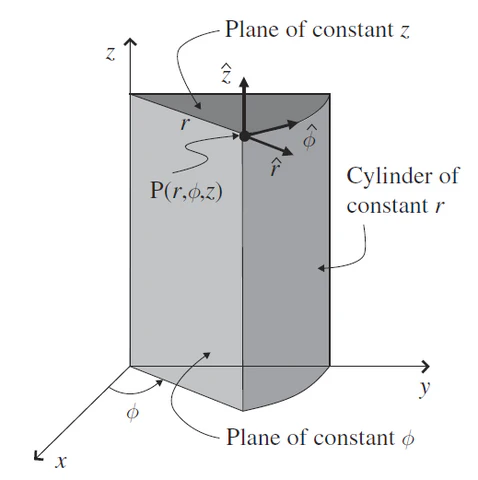
\includegraphics[width=8cm]{Figuras/Lineas-coordenadas-cilindricas.png}
    \caption{Sistema coordenado cilíndrico. Se puede apreciar que un punto en este es completamente determinado por la intersección de dos planos ($z =$ constante y $\phi = $ constante) y una superficie cilíndrica ($\rho = $ constante). Además, es posible apreciar la dirección de los tres vectores unitarios, $\hat{e}_\rho = \hat{\rho}$, $\hat{e}_\phi = \hat{\phi}$ y $\hat{e}_z = \hat{z}$.}
\end{figure}


\subsection{Coordenadas esféricas}

En coordenadas esféricas $(r, \theta, \phi)$, el vector posición de un punto con coordenadas cartesianas $(x,y,z)$ puede representarse como 
\begin{equation}
    \x = r \cos \phi \sin \theta \hat{\imath} + r \sin \phi \sin \theta \hat{\jmath} + r \cos \theta \hat{k} \ ,
\end{equation}
de donde se deduce que la relación entre ambos sistemas es 
\begin{equation}
    \begin{array}{rcl}
        x & = & r \cos \phi \sin \theta \ , \\
        y & = & r \sin \phi \sin \theta \ , \\
        z & = & r \cos \theta \ ,
    \end{array}
\end{equation} 
donde $\rho \in [0, +\infty)$, $\phi \in [0, 2\pi]$, y $\theta \in [0, \pi]$.
% , o inversamente,
% \begin{equation}
%     \begin{array}{rcl}
%         \rho & = & \sqrt{x^2 + y^2 + z^2} \ , \\
%         \theta & = & \tan^{-1}\left(\frac{y}{x}\right) \ , \\
%         \phi & = & z \ .
%     \end{array}
% \end{equation} 

A partir del vector posición, podemos obtener los vectores direccionales 
\begin{align}
    \vec{e}_r & = \frac{\partial \x}{\partial r} = \sin \theta \cos \phi \hat{\imath} + \sin \theta \sin \phi \hat{\jmath} + \cos \theta \hat{k} \ , \\
    \vec{e}_\theta & = \frac{\partial \x}{\partial \theta} = r \cos \phi \cos \theta \hat{\imath} + r \sin \theta \cos \theta \hat{\jmath} - r \sin \theta \hat{k} \ , \\
    \vec{e}_\phi & = \frac{\partial \x}{\partial \phi} = -r \sin \theta \sin \phi  \hat{\imath} + r \sin \theta \cos \phi \hat{\jmath} \ ,
\end{align}
con respectivos factores de escala 
\begin{equation}
    h_r = 1 \, , \quad h_\theta = r \, , \quad h_\phi = r \sin \theta \ .
\end{equation}

Un elemento de longitud será dado por 
\begin{equation}
    d\x(r, \theta, \phi) = dr \hat{e}_r + r d\theta \hat{e}_\theta + r \sin \theta d\phi \hat{e}_\phi \ ,
\end{equation}
y un elemento de volumen será
\begin{equation}
    dV(\rho, \phi, z) = r^2 \sin \theta dr d\theta d\phi \ .
\end{equation}

\begin{figure}[htbp]
    \centering
    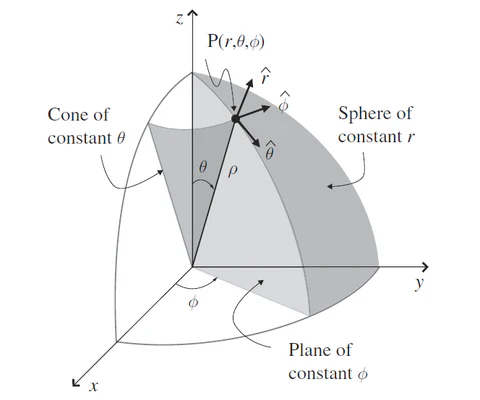
\includegraphics[width=8cm]{Figuras/Lineas-coordenadas-esfericas.png}
    \caption{Sistema coordenado esférico. Se puede apreciar que un punto en este es completamente determinado por la intersección de un ($\phi = $ constante), una superficie cónica ($\theta = $ constante) y una superficie esférica ($r = $ constante). Además, es posible apreciar la dirección de los tres vectores unitarios, $\hat{e}_r = \hat{r}$, $\hat{e}_\theta = \hat{\theta}$ y $\hat{e}_\phi = \hat{\phi}$.}
\end{figure}

\section{El operador Nabla}

Existen algunas operaciones diferenciales que puedes ser desarrolladas en campos escalares y vectoriales, y tienen una variedad de aplicaciones en física. Las tres más importantes corresponden al \emph{gradiente} de un campo escalar, la \emph{divergencia} de un campo vectorial, y el \emph{rotacional} de un campo vectorial.

Definiremos estas operaciones desde el punto de vista matemático, pues si bien pueden obtenerse a partir de nociones físicas y geométricas, en honor al tiempo no será posible hacer esta revisión. Para más detalles de estas, puede ver el capítulo 11 de Riley \cite{Riley}, o el capítulo 5 de Barea \cite{Barea}.

\begin{defi}
    Se define el operador \textbf{nabla} (o \emph{del} en inglés) en coordenadas cartesianas como 
    \begin{equation}
        \nabla \equiv \hat{\imath} \frac{\partial}{\partial x} + \hat{\jmath} \frac{\partial}{\partial y} + \hat{k} \frac{\partial}{\partial z} \ .
    \end{equation}
\end{defi}

\subsection{Gradiente}

\begin{defi}
    El \textbf{gradiente de un campo escalar}, $\nabla \phi \equiv \operatorname{grad}\phi$, corresponde a la operación que entrega como resultado la dirección \emph{de mayor cambio} en el campo $\phi$.

    En el caso que el campo sea constante (como un plano), entonces el gradiente corresponde al vector \emph{perpendicular} a la superficie definida por el campo $\phi$. 
\end{defi}

\begin{figure}[htbp]
    \centering
    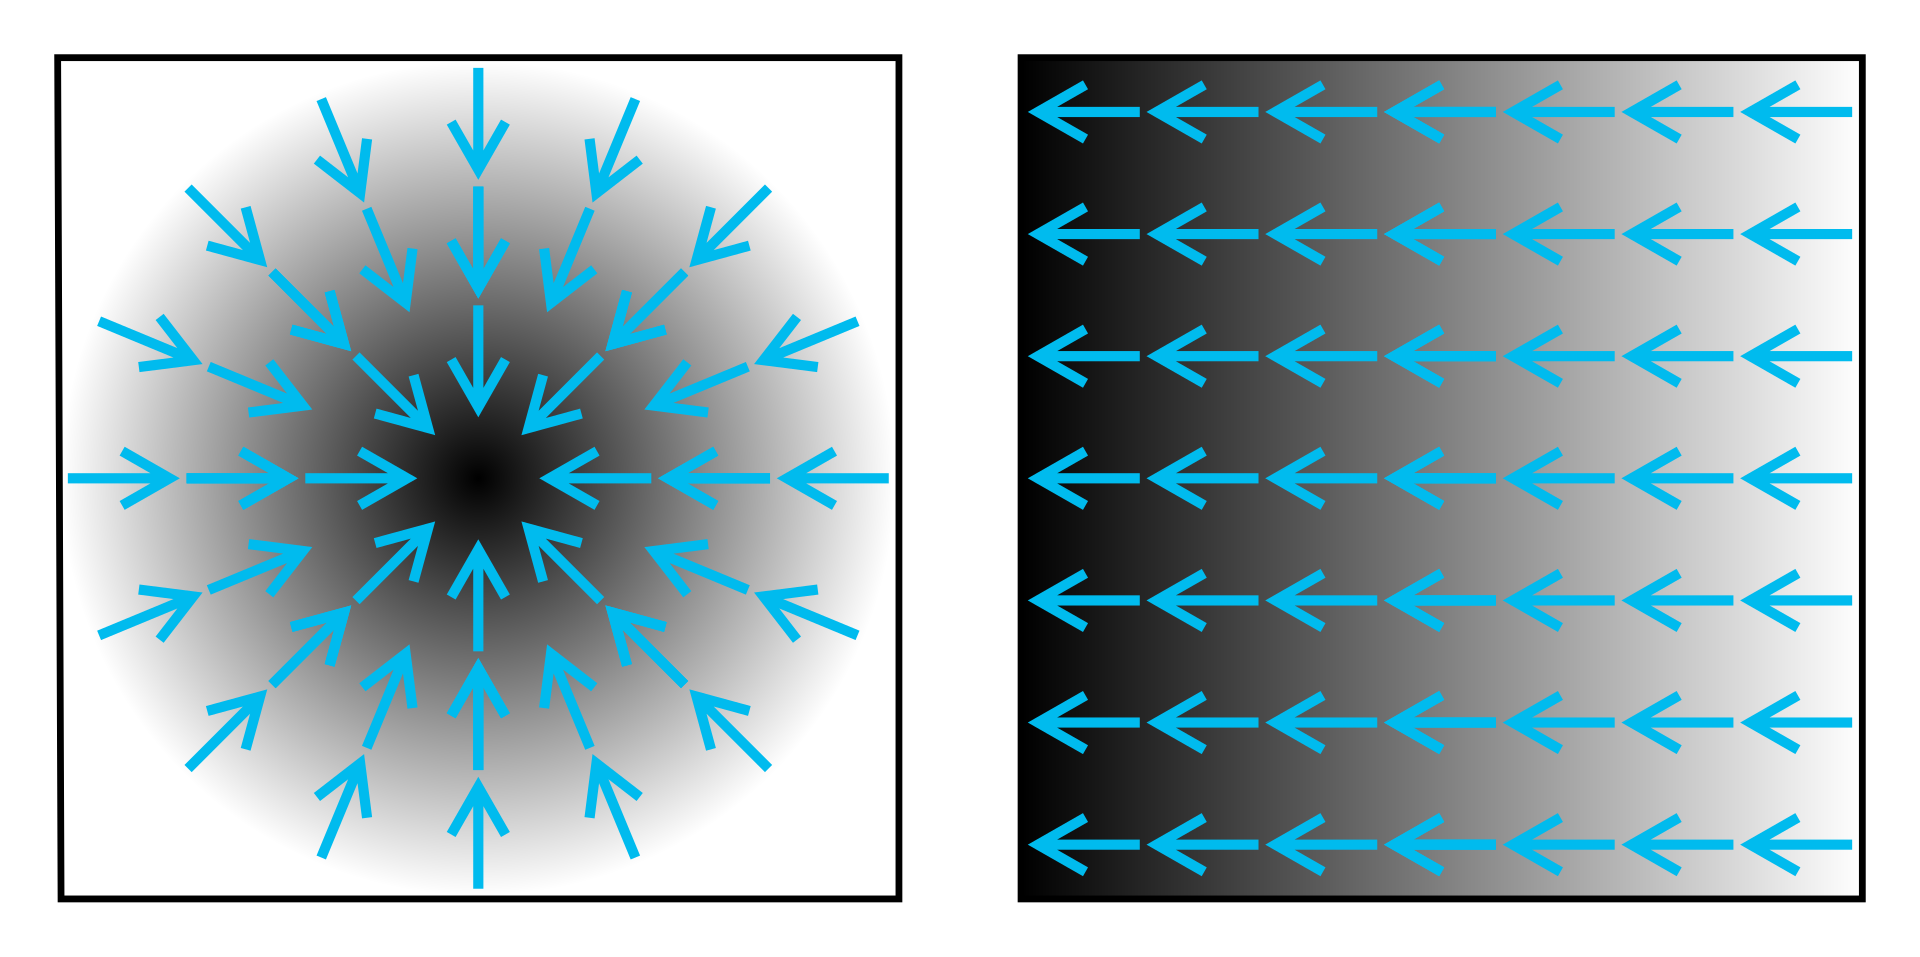
\includegraphics[width=12cm]{Figuras/Gradiente.png}
    \caption{Ilustración del concepto de gradiente. Nuestro campo escalar es representado por la escala de grises, donde un color más oscuro denota un mayor valor. Las flechas indican la dirección del gradiente en cada punto donde ellas aparecen, el que siempre apunta en la dirección de mayor cambio en la intensidad de la escala.}
\end{figure}

En coordenadas cartesianas, el gradiente puede escribirse como 
\begin{equation}
    \nabla \phi = \hat{\imath} \frac{\partial \phi}{\partial x} + \hat{\jmath} \frac{\partial \phi}{\partial y} + \hat{z} \frac{\partial \phi}{\partial z} \ ,
\end{equation}
mientras que en un sistema curvilíneo ortogonal podrá representarse como 
\begin{equation}
    \nabla \psi = \hat{e}_1 \frac{1}{h_1} \frac{\partial \psi}{\partial q_1} + \hat{e}_2 \frac{1}{h_2} \frac{\partial \psi}{\partial q_2} + \hat{e}_3 \frac{1}{h_3} \frac{\partial \psi}{\partial q_3} \ .
\end{equation}

Podemos representar cambios infinitesimales en el campo $\phi$, por ejemplo entre dos puntos $Q = (x_Q, y_Q, z_Q)$ y $P = (x_P, y_P, z_P)$ infinitesimalmente cercanos, mediante el diferencial $d\phi$:
\begin{equation*}
    d\phi = \phi(Q) - \phi(P) = \phi(x_Q, y_Q, z_Q) - \phi(x_P, y_P, z_P) = \frac{\partial \phi}{\partial x} dx + \frac{\partial \phi}{\partial y} dy + \frac{\partial \phi}{\partial z} dz \ ,
\end{equation*}
donde $d\x = (dx, dy, dz) = (x_Q - x_P, y_Q - y_P, z_Q - z_P)$ representa un vector que conecta por puntos $P$ y $Q$.

Notemos que 
\begin{equation*}
    d\phi = \nabla \phi \cdot d\x \ ,
\end{equation*}
donde $\theta$ es el ángulo que forman los vectores $\nabla \phi$ y $d\x$. Integremos ambos lados de la igualdad a lo largo de una curva que una los puntos $P$ y $Q$. Para el lado izquierdo, tenemos que
\begin{equation*}
    \int_P^Q d\phi = \phi(x_Q, y_Q, z_Q) - \phi(x_P, y_P, z_P) \ ,
\end{equation*}
por lo que en la igualdad resultará en 
\begin{equation}
    \int_P^Q d\phi = \int_C \nabla \phi \cdot d\x = \phi(x_Q, y_Q, z_Q) - \phi(x_P, y_P, z_P) \ ,
\end{equation}
de modo que la segunda integral, que es una integral de línea, \emph{no depende del camino seguido, sino únicamente de los puntos de inicio y término}.

\begin{defi}
    Decimos que un campo vectorial es \textbf{conservativo} si la integral de línea entre los puntos $A$ y $B$ es independiente del camino escogido entre ambas.
\end{defi}

Por ello, el gradiente de un campo escalar es un campo vectorial conservativo.

\subsection{Divergencia}

\begin{defi}
    Se define la \textbf{divergencia de un campo vectorial}, $\nabla \cdot \vec{A} = \operatorname{div} \vec{A}$ como una medida del flujo neto del campo $\vec{A}$ a través de una superficie cerrada.
\end{defi}

En coordenadas cartesianas, la divergencia viene dada por
\begin{equation}
    \nabla \cdot \vec{A} = \frac{\partial A_x}{\partial x} + \frac{\partial A_y}{\partial y} + \frac{\partial A_z}{\partial z} \ ,
\end{equation}
mientras que en coordenadas curvilíneas ortogonales puede representarse como 
\begin{equation}
    \nabla \cdot \vec{A} = \frac{1}{h_1 h_2 h_3} \left( \frac{\partial(h_2 h_3 C_1)}{\partial q_1} + \frac{\partial(h_1 h_3 C_2)}{\partial q_2} + \frac{\partial(h_1 h_2 C_3)}{\partial q_3} \right) \ ,
\end{equation}
donde en el sistema coordenado, $\vec{A} = (A_1, A_2, A_3)$.

Siguiendo la interpretación de la divergencia como un flujo, tendremos que si $\nabla \cdot \vec{A} > 0$, diremos que existe una \textbf{fuente} de líneas de campo en dicha región. En cambio, cuando $\nabla \cdot \vec{A} < 0$, diremos que existe un \textbf{sumidero} en la región.

\begin{defi}
    Dado un campo vectorial $\vec{A}(\x)$, decimos que este es \textbf{solenoidal} si 
    \begin{equation}
        \nabla \cdot \vec{A} = 0 \ .
    \end{equation}
\end{defi}

\begin{ejemplo}
    La divergencia del vector posición puede obtenerse fácilmente en coordenadas cartesianas, de modo que 
    \begin{equation}
        \nabla \cdot \x = \frac{\partial x}{\partial x} + \frac{\partial y}{\partial y} + \frac{\partial z}{\partial z} = 3 \ .
    \end{equation}

    Dado que la divergencia de un vector es un escalar, este resultado es válido \textbf{para cualquier sistema de coordenadas}.
\end{ejemplo}

% \subsection{Teorema de Gauss, o de la divergencia}

Relacionado a la divergencia de un campo vectorial, existe un teorema que nos permite establecer una equivalencia entre integrales de superficie sobre una superficie $S$ cerrada, y una integral de volumen sobre la región $V$ encerrada por $S$.

\begin{teorema}{\textbf{(Teorema de la divergencia, o de Gauss).}} \marginnote{Teorema de Gauss}
    Dado un campo vectorial $\vec{A}(\x)$, continuo y diferenciable, la integral de su divergencia sobre una región $V$ es igual a la integral de superficie de la componente normal de $\vec{A}(\x)$ sobre la superficie $S$ que encierra a la región $V$:
    \begin{equation}
        \oint_S \vec{A}(\x) \cdot d\vec{S} = \int_V \nabla \cdot \vec{A}(\x) \, dV \ .
    \end{equation}
\end{teorema}

\begin{ejemplo}
    Siguiendo con el resultado obtenido en el ejemplo anterior, podemos utilizar el teorema de Gauss para una región $R$ arbitraria encerrada por una superficie $S$, gracias a lo cual obtenemos que 
    \begin{equation*}
        \oint_S \x \cdot d\vec{S} = \int_R \nabla \cdot \x \, dV = \int_R 3 \, dV = 3V \,
    \end{equation*}
    donde $V$ es el volumen de la región $R$. Reordenando términos, podemos concluir que el volumen de esta región se puede obtener como 
    \begin{equation}
        V = \frac{1}{3} \oint_S \x \cdot d\vec{S} \ .
    \end{equation}
\end{ejemplo}

\subsection{Rotacional}

\begin{defi}
    El \textbf{rotacional de un campo vectorial}, $\nabla \times \vec{A} = \operatorname{rot} \vec{A} = \operatorname{curl} \vec{A}$, correesponde a una medida de la \emph{densidad de circulación} de $\vec{A}$ alrededor de una curva $C$, que encierra una superficie $S$.

    De forma más coloquial, el rotacional mide la \emph{tendencia del campo a inducir una rotación alrededor de un punto} $\x$.
\end{defi}

En coordenadas cartesianas, este toma la forma 
\begin{align}
    \nonumber \nabla \times \vec{A} & = \left( \frac{\partial A_z}{\partial y} - \frac{\partial A_y}{\partial z} \right) \hat{\imath} + \left( \frac{\partial A_x}{\partial z} - \frac{\partial A_z}{\partial x} \right) \hat{\jmath} + \left( \frac{\partial A_y}{\partial x} - \frac{\partial A_x}{\partial y} \right) \hat{k} \\
    & = \left|
    \begin{array}{ccc}
        \hat{\imath} & \hat{\jmath} & \hat{k} \\
        \dfrac{\partial}{\partial x} & \dfrac{\partial}{\partial y} & \dfrac{\partial}{\partial z} \\
        A_x & A_y & A_z \\
    \end{array}
    \right| \ ,
\end{align}
o en coordenadas curvilíneas generalizadas,
\begin{equation}
    \nabla \times \vec{A} = \frac{1}{h_1 h_2 h_3} \left| 
    \begin{array}{ccc}
        h_1 \hat{e_1} & h_2 \hat{e}_2 & h_3 \hat{e}_3 \\
        \dfrac{\partial}{\partial q_1} & \dfrac{\partial}{\partial q_2} & \dfrac{\partial}{\partial q_3} \\
        h_1 A_1 & h_2 A_2 & h_3 A_3 \\
    \end{array}
    \right| \ .
\end{equation}

\begin{defi}
    Dado un campo vectorial $\vec{A}(\x)$, decimos que este es \textbf{irrotacional} si 
    \begin{equation}
        \nabla \times \vec{A} = 0 \ .
    \end{equation}
\end{defi}

% \subsection{Teorema de Stokes, o del rotacional}

De forma similar al teorema de Gauss, el teorema de Stokes es una forma de conectar una integral de línea de un campo $\vec{V}(\x)$ a lo largo de una curva cerrada $C$ con la integral de superficie del rotacional de $\vec{A}(\x)$ sobre la superficie $S$ encerrada por $C$.

\begin{teorema}{\textbf{(de Stokes, o del rotacional).}} \marginnote{Teorema de Stokes}
    Consideremos un campo vectorial $\vec{A}(\x)$ continuo y diferenciable. Entonces, la integral de línea alrededor de una curva cerrada $C$ es igual a la integral de superficie de la componente normal de su rotacional sobre cualquier superficie $S$ limitada por la curva $C$:
    \begin{equation}
        \oint_C \vec{A}(\x) \cdot d\x =  \int_S \left( \nabla \times \vec{A}(\x) \right) \cdot \, d\vec{S} \ .
    \end{equation}
\end{teorema}

En este caso, los diferenciales $d\x$ y $d\vec{S}$ están relacionados entre sí. Una vez fijamos el sentido en que recorreremos el contorno utilizando el vector $d\x$, podemos notar que este es un vector tangente a la superficie $S$. Viendo la figura X, observamos que existen solo dos posibles vectores perpendiculares a $d\x$ que a su vez sean tangentes a $S$: uno que apunta hacia la superficie, que llamaremos $d\x'$, y uno que no lo hace. Teniendo esto en cuenta, el vector $d\vec{S}$ puede ser obtenido como 
\begin{equation*}
    d\vec{S} = d\x \times d\x' \ ,
\end{equation*}
es decir, debe seguir el sentido establecido por la \textbf{regla de la mano derecha}.

\subsection{Identidades vectoriales}

Dados los campos escalares $\phi$ y $\psi$, y los campos vectoriales $\vec{A}$ y $\vec{B}$, algunas identidades que surgen de la aplicación del operador nabla sobre sumas o productos de estos campos son las siguientes:
\begin{itemize}
    \item $\nabla (\phi + \psi) = \nabla \phi + \nabla \psi$.
    \item $\nabla \cdot \left( \vec{A} + \vec{B} \right) = \nabla \cdot \vec{A} + \nabla \cdot \vec{B}$.
    \item $\nabla \times \left( \vec{A} + \vec{B} \right) = \nabla \times \vec{A} + \nabla \times \vec{B}$.
    \item $\nabla(\phi \psi) = \phi \nabla \psi + \psi \nabla \phi$.
    \item $\nabla \cdot \left( \phi \vec{A} \right) = \phi \nabla \cdot \vec{A} + \vec{A} \cdot \nabla \phi$.
    \item $\nabla \cdot (\vec{A} \times \vec{B}) = \vec{B} \cdot (\nabla \times \vec{A}) - \vec{A} \cdot (\nabla \times \vec{B})$.
    \item $\nabla \times (\phi \vec{A}) = \nabla \phi \times \vec{A} + \phi \nabla \times \vec{A}$.
    \item $\nabla(\vec{A} \cdot \vec{B}) = \vec{A} \times (\nabla \times \vec{B}) + \vec{B} \times (\nabla \times \vec{A}) + (\vec{A} \cdot \nabla) \vec{B} + (\vec{B} \cdot \nabla) \vec{A}$,
    donde 
    \begin{equation*}
        \vec{A} \cdot \nabla = A_x \frac{\partial}{\partial x} + A_y \frac{\partial}{\partial y} + A_z \frac{\partial}{\partial z} \ .
    \end{equation*}
\end{itemize}


De igual forma, podemos estudiar las aplicaciones sucesivas del operador nabla sobre campos escalares o vectoriales. Enumeraremos únicamente aquellas cantidades que sí tiene sentido definir:
\begin{itemize}
    \item \textbf{Divergencia de un gradiente}, $\nabla \cdot (\nabla \phi) = (\nabla \cdot \nabla) \phi = \nabla^2 \phi$, operación que es conocida como \textbf{laplaciano} de un campo escalar. En coordenadas curvilíneas ortogonales,
    \begin{equation}
        \nabla^2 \phi = \frac{1}{h_1 h_2 h_3}\left[ \frac{\partial}{\partial q_1} \left( \frac{h_2 h_3}{h_1} \frac{\partial \phi}{\partial q_1} \right) + \frac{\partial}{\partial q_2} \left( \frac{h_1 h_3}{h_2} \frac{\partial \phi}{\partial q_2} \right) + \frac{\partial}{\partial q_3} \left( \frac{h_1 h_2}{h_3} \frac{\partial \phi}{\partial q_3} \right) \right] \ .
    \end{equation}
    \item \textbf{Rotacional de un gradiente}, $\nabla \times (\nabla \phi) = 0$, pues las derivadas parciales cruzadas que surgirán se cancelarán entre sí. En consecuencia, todo gradiente es irrotacional.
    \item \textbf{Gradiente de una divergencia}, $\nabla (\nabla \cdot \vec{A})$.
    \item \textbf{Divergencia de un rotacional}, $\nabla \cdot (\nabla \times \vec{A}) = 0$, donde nuevamente las derivadas parciales cruzadas se anularán. En consecuencia, todo rotacional es solenoidal.
    \item \textbf{Rotacional de un rotacional}, $\nabla \times (\nabla \times \vec{A}) = \nabla (\nabla \cdot \vec{A}) - \nabla^2 \vec{A}$.
\end{itemize}

% \section{Teoremas integrales}


\section{Teoría del potencial}

Cerramos este capítulo explicando la importancia de los resultados aquí descritos. Consideremos un campo escalar $\phi(\x)$. Al calcular su gradiente, obtenemos un campo vectorial, que llamaremos $\vec{F}(\x) = \nabla \phi(\x)$. De aquí, podemos inferir dos resultados:
\begin{enumerate}
    \item El campo vectorial resultante es irrotacional, pues $\nabla \times \vec{F} = \nabla \times (\nabla \phi) = 0$.
    \item Por definición, $\vec{F} \cdot d\x = \nabla \phi \cdot d\x = d\phi$, de modo que para cualquier curva cerrada, $\oint_C \vec{F} \cdot d\x = \oint_C d\phi = 0$.
\end{enumerate}

Del segundo resultado, podemos concluir que \emph{la integral de línea de} $\vec{F}$ \emph{a lo largo de cualquier trayectoria que una los puntos} $A$ y $B$ \emph{proporciona siempre el mismo valor, y es independiente de la trayectoria escogida}. Nos referiremos a este comportamiento diciendo que el campo $\vec{F}(\x)$ es \textbf{conservativo}.

\begin{teorema}
    Dado un campo vectorial $\vec{F}(\x)$, son equivalentes las tres afirmaciones:
    \begin{itemize}
        \item $\vec{F}(\x)$ es un campo conservativo.
        \item $\vec{F}(\x)$ es irrotacional.
        \item Existe un campo escalar $\phi$, denominado \textbf{potencial escalar}, tal que $\vec{F}(\x) = - \nabla \phi$.
    \end{itemize}
\end{teorema}

Ejemplos del resultado de este teorema son:
\begin{itemize}
    \item El campo eléctrico, $\vec{E}$, que se puede definir a partir de un potencial electrostático $\phi$, tal que $\vec{E} = - \nabla \phi$.
    \item Toda fuerza $\vec{F}$, que se encuentre asociada a una energía potencial $U$, tal que $\vec{F} = - \nabla U$. Algunas de ellas son la fuerza elástica, la fuerza gravitacional o la fuerza eléctrica.
\end{itemize}

\subsection{Teorema de Helmholtz}

Bajo ciertas condiciones, el resultado obtenido anteriormente no será suficiente. En dichas condiciones, es posible definir una construcción más complicada utilizando el siguiente teorema.

\begin{teorema}{\textbf{(de Helmholtz).}}
    Sea $\vec{V}(\x)$ un campo vectorial diferenciable, con derivadas parciales continuas, y cuya divergencia y rotacional se anulan en el límite $|\x| \to \infty$. Entonces, podemos descomponer $\vec{V}$ en una componente \emph{irrotacional}, y en una componente \emph{solenoidal}, dependientes de un \textbf{potencial escalar} $\phi$ y un \textbf{potencial vectorial} $\vec{A}$, respectivamente:
    \begin{equation}
        \vec{V} = -\nabla \phi + \nabla \times \vec{A} \ ,
    \end{equation}
    donde
    \begin{align}
        \phi(\x)    & = \frac{1}{4\pi} \int_V \frac{\nabla \cdot \vec{V}(\x')}{|\x-\x'|} \, dV' \ , \\
        \vec{A}(\x) & = \frac{1}{4\pi} \int_V \frac{\nabla \times \vec{V}(\x')}{|\x-\x'|} \, dV' \ . 
    \end{align}
\end{teorema}

\begin{corolario}
    Un campo vectorial $\vec{J}(\x)$ solenoidal, puede representarse en términos de un potencial vector $\vec{A}$, tal que 
    \begin{equation}
        \vec{J}(\x) = \nabla \times \vec{A} \ .
    \end{equation}
\end{corolario}